%!TEX root = thesis_cgo.tex
\chapter{Conformational analysis of the $\gamma$-Tubulin carboxyl terminus}

In this chapter we discuss the impact of local charge on the global dynamics of the $\gamma$-Tubulin C-terminus (\gct). In order to measure how the addition of local negative charge in an acidic polypeptide affects the conformational sampling of the \gct, we simulated the dynamics of various isoforms of the \gct using MD. By comparing results from our simulations to experimental measurements performed with NMR spectroscopy on the \gct, we were able to propose that local changes in charge at specific residues in the polypeptide have the ability to bias the conformational sampling of the \gct in such a way that may be regulating the availability of binding surfaces on $\gamma$-Tubulin.

\section{NMR}
Talk about NMR stuff here.
`
\section{Setting up the MD runs}

Molecular Dynamics simulations (MDS) on WT and Y11D \gct s were carried out using MPI-enabled GROMACS 4.6.6 software\cite{hess2008gromacs} and a CentOS 5 high performance computational cluster. Calculations were distributed over 64 Dual Sandy Bridge 8-core, 2.6 GHz computing nodes and run under periodic boundary conditions with the OPLS-AA (Optimized Potential for Liquid Simulations ? All Atom) force field ~\cite{kaminski2001evaluation}.  The starting \gct polypeptide configurations were obtained from secondary and tertiary structure predictions by RaptorX \cite{kallberg2012template} and solvated using the SPCE (extended single point charge) water model in a dodecahedral box while enforcing a minimum distance between the edge of the box and solute of 1 nanometer. The total charge of the system was neutralized by adding sodium ions to the solution. Energy minimization was carried out using a steepest descent algorithm for a maximum of 50,000 steps until a maximum force of 100 kJ/mol between atoms was achieved. A 1 nm cut-off was used for non-bonded interactions, and long-range electrostatics were calculated using a Particle Mesh Edwald Sum algorithm. The systems equilibrated under the constant NVT and NPT ensembles (288K and 1 atm) for 5 ns before the production 2 $\mu$s simulations. Post-processing of all trajectories was done using the \texttt{trjconv} module of GROMACS. Theoretical random-coil structural ensembles (10,000 conformers) were calculated based on the \gct primary amino acid sequence using Flexible Meccano software \cite{ozenne2012flexible}. Translational diffusion coefficients were calculated for each structure using hydroNMR software \cite{de2000hydronmr}. 
MD conformations were grouped into percentile classes based on radius of gyration (Rg) computed using the GROMACS \texttt{g\_gyrate} module. Each Rg percentile group was represented by the three structures with lowest root-mean-squared-difference RMSD values to all other structures, calculated using the GROMACS \texttt{g\_rms} module. Atomic distance matrices were calculated using the GROMACS \texttt{g\_mdmat} module.

\section{Conformational sampling of \gct isoforms}

Our NMR experiments provide evidence for a major alteration in the global dynamics of the \gct in the presence of the Y11D mutation characterized by collective motions involving the entire polypeptide chain occurring on the microsecond timescale. We then asked whether this phenomenon can be reproduced \textit{in silico} using MDS.  If we are able to reproduce the transition \textit{in silico}, the resulting MD data can be used to obtain additional insight into the structural characteristics of the conformational sampling of the \gct at an atomic resolution. We computed trajectories for the WT and Y11D \gct polypeptides by running independent 2$\mu$s GROMACS simulations, and computed the translational diffusion coefficient from the resulting MDS structural trajectories at 1 ns time steps \figref{dc}. We found that the diffusion coefficient (\diffusion) of the WT \gct remains relatively constant over the total simulation time (\diffusion = \num{1.237e-6} $\pm$ \SI{1.5816e-8}{\dcunits} and agrees well with the NMR-derived value (\diffusion=\num{1.25e-6} $\pm$  \SI{1e-8}{\dcunits}.  Similarly to what was seen by NMR, we find that the mean \diffusion of the Y11D \gct polypeptide is slightly lower than that of the WT \gct (\diffusion= \num{1.224e-6} $\pm$ \SI{3.503e-8}{\dcunits}). These results confirm that the \gct, while disordered, is more compact than a fully denatured polypeptide chain. Interestingly, between \num{762} to \SI{1255}{\ns} in the MDS, the Y11D \gct underwent transient excursions to less compact con-formations with significantly lower diffusion coefficients (mean \diffusion= \num{1.152e-6} $\pm$ \SI{2.0325e-8}{\dcunits}). This sub-population is more ex-tended (i.e. diffuses more slowly) than any conformation sampled by the WT \gct throughout the entire MDS. While the Y11D \gct extended states do not overlap with the conformational ensemble of the WT \gct polypeptides, they do, however, lie within the conformational space expected for a typical random-coil poly-peptide, as modeled by an ensemble of 10,000 disordered extended conformers (Fig. S8) derived from the \gct primary sequence using the \texttt{Flexible Meccano} tool.  

\begin{figure}
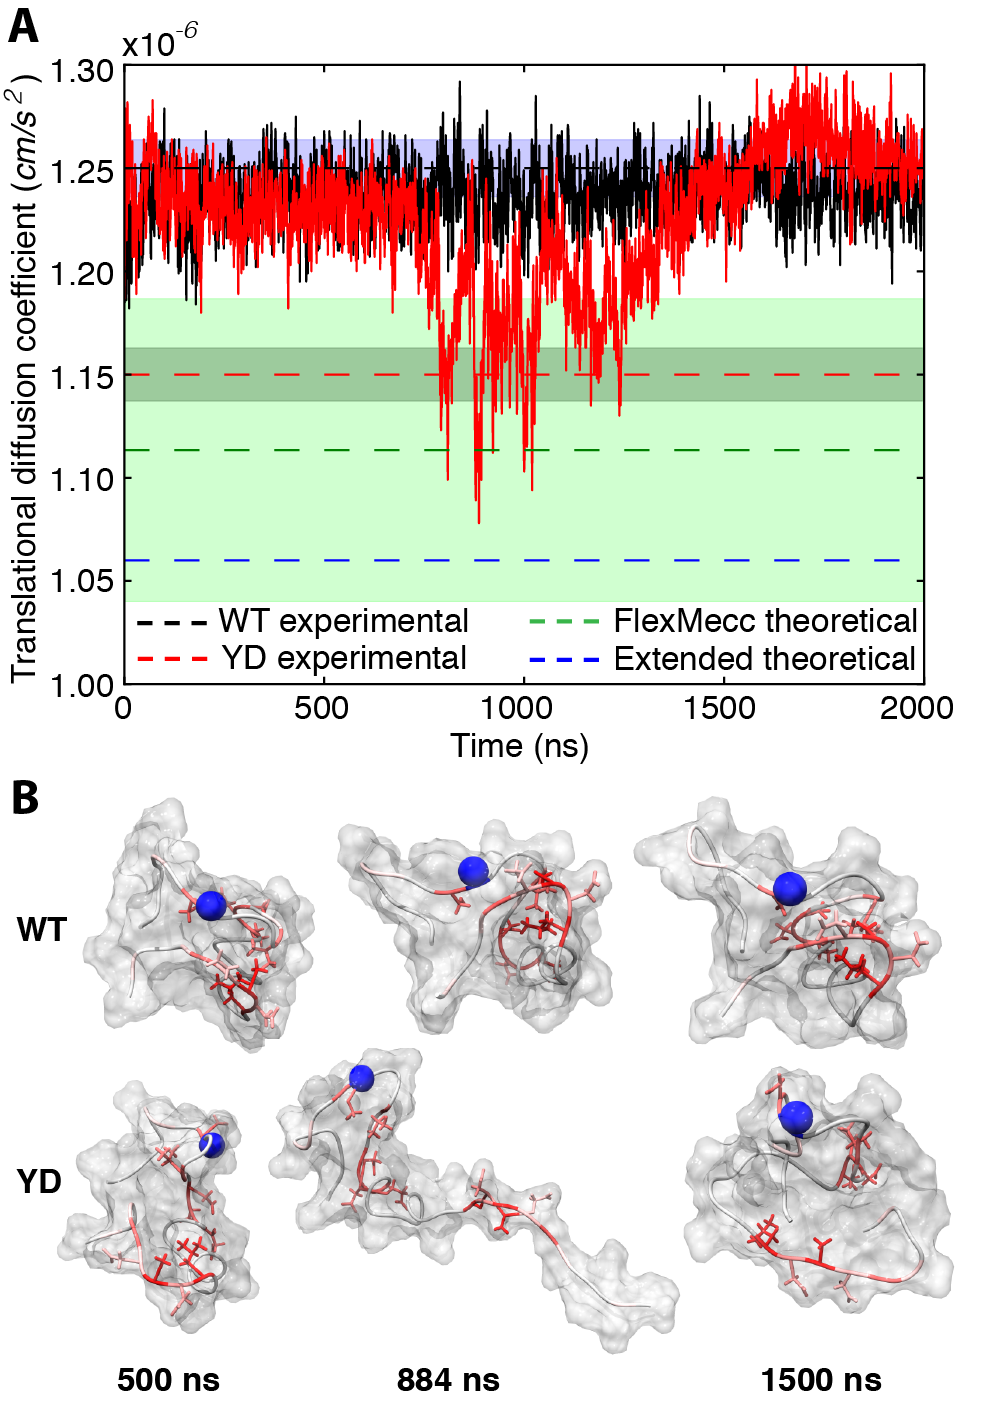
\includegraphics{figures/Figure_7.png}
\label{dc}
\caption{Diffusion Coefficient}
\end{figure}

In order to obtain an initial visualization of the transient opening motions experienced by the Y11D polypeptide, we extracted struc-tural models from the simulation at the time step with the lowest value of Ds for the Y11D \gct polypeptide (\SI{844}{\ns}; \diffusion= \SI{1.078e-6}{\dcunits}) as well as the time steps at \SI{500}{\ns} (\diffusion=\SI{1.268e-6}{\dcunits} for WT and \SI{1.235e-6}{\dcunits} for Y11D) and \SI{1500}{\ns} (\diffusion=\SI{1.233e-6}{\dcunits} for WT and \SI{1.241e-6}{\dcunits}s for Y11D). The expansion experienced by the Y11D polypeptide is clearly observed in the \SI{844}{\ns} structure. We hypothesize that the global microsecond dynamics characterized by NMR for the Y11D \gct  correspond to the transient opening motions seen by MDS, with the major state corresponding to the compact form and the minor state corresponding to the expanded form. Residues with large-magnitude dispersion profiles (i.e. those in Figure 6 with large $\Delta$R2) have chemical shifts that are quite different in the major and the minor states. If the NMR dynamics correspond to transient expansion, these residues should experience different local environments in the collapsed and expanded states. Residues with large $\Delta$R2 values (coloured red in Figure 7B) indeed are located in a compact cluster at 500 ns for the Y11D \gct and at all time steps for the WT \gct. However during expansion, this cluster dissociates and the residues become more solvent-exposed. This provides a possible explanation for how residues throughout a disordered polypeptide can experience a concerted, two-state, dynamical process presence of the Y11D mutation, and suggests that it is the separation of a cluster of residues located in N and C termini of the \gct  polypeptide that drives a transition to extended conformations with a concomitant  reduction of the translational diffusion coefficient.

\begin{figure}
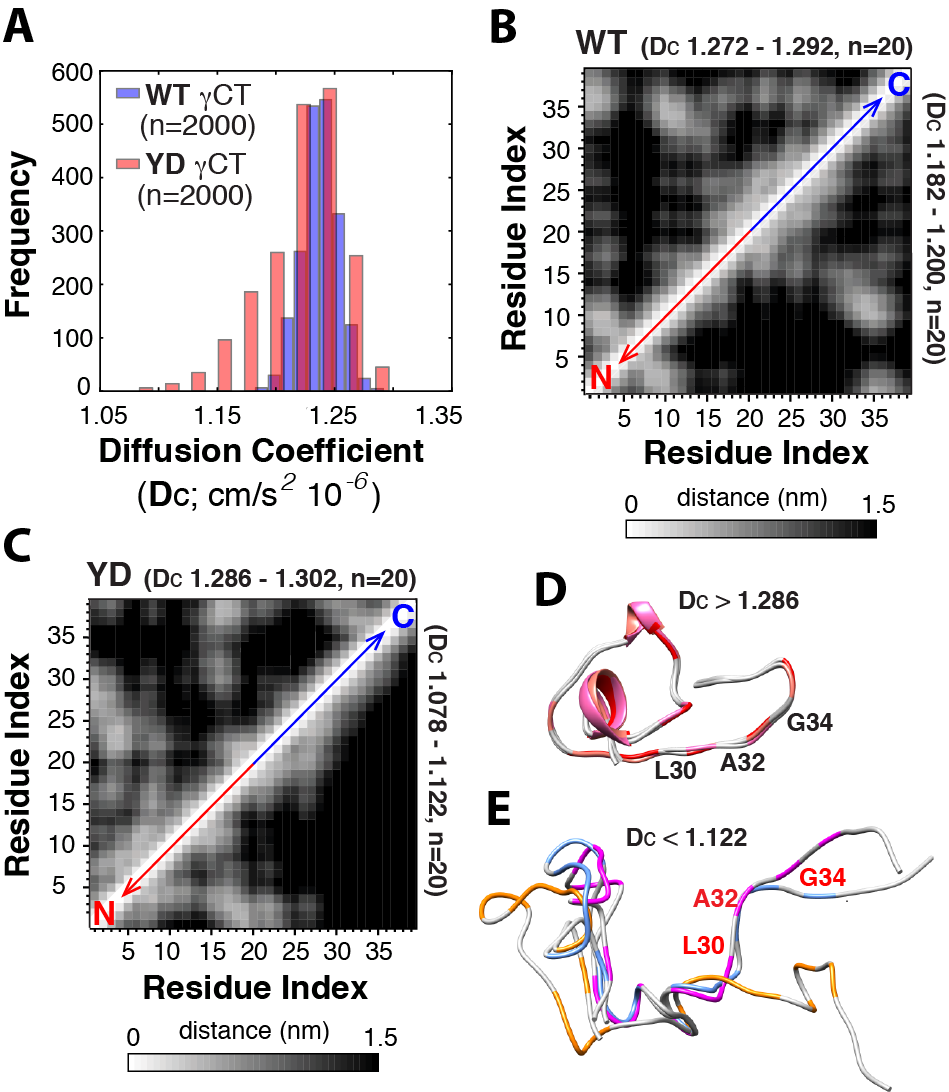
\includegraphics{figures/Figure_8_Dc_version.png}
\label{contacts}
\caption{Contact Maps}
\end{figure}

	To further characterize the transition observed in the Y11D \gct polypeptide, we chose a subset of 2000 time steps (every 1 ns) for additional analysis.  We calculated theoretical diffu-sion coefficients for each structure, yielding the frequency histo-grams  shown Figure 8A. The Y11D \gct distribution is clearly skewed compared to that of the WT with many structures exhibit-ing far slower self-diffusion and more extended conformations. The conformations within the top and bottom 1\% (20 structures each) of the WT \gct and Y11D \gct Ds distributions best represent the collapsed (top 1\%) and extended (bottom 1\%) conformations for \gct polypeptides. In the case of the WT, we do not expect the upper and lower Ds subsets to substantially differ, as the WT \gct conformations exhibit fairly homogenous compactness overall. For Y11D \gct, we expect the upper Ds subset to resemble that of the WT \gct, while the lower Ds subset is expected to reflect the tran-sient opening process. We plotted the mean distance between alpha carbons of all pairs of residues for as contact maps for the set of collapsed (upper) and extended (lower) conformations of the WT \gct polypeptide (Fig. 8B) and the Y11D \gct polypeptide (Fig. 8C).   As expected, the upper and lower Ds subsets of the WT \gct and the upper Ds subset of the Y11D \gct polypeptides show similar patterns of pair-wise contacts.  In contrast, the C-terminal residues in the lower Ds subset of the Y11D \gct lose the majority of contacts with N terminal residues, as a consequence of the conformational expansion. Next, we isolated the three confor-mations from the upper and lower Ds subsets of  Y11D \gct poly-peptides with the lowest all-to-all RMS, also known as centroid structures, shown in Fig. 8D,E. with large relaxation dispersion magnitudes indicated in red. This analysis shows that the extended conformations consist of a compact N-terminus with residues lo-cated in the C-terminal region of the \gct, (including dynamical-ly-broadened residues L30, A32 and G34) isolated from the N-terminus and solvent-accessible. Through MDS we are able to re-produce the anomalously rapid diffusion (i.e. high compactness) of the WT and Y11D ground-state \gct polypeptides. Moreover, we saw that the Y>D substitution caused relatively slow collective motions of the entire polypeptide chain, as observed by NMR.
 

Representative structures obtained identifying structures with lowest all-to-all RMSD values for the YD high diffusion coefficient group (D) and YD low diffusion coefficient group (E), residues with $\Delta$R2 val-ues greater than 5 s-1 are labeled in red.
	Our experimental analysis of the structural properties of the \gct using NMR and corresponding MDS are based on the properties of the WT and Y11D \gct polypeptides in isolation. In order to determine whether the conformations and dynamics we observed for the isolated ??CTs are physically consistent within the context of the full-length $\gamma$-tubulin protein, we docked the min-imum Ds \gct model (Fig. S9) onto the globular domain of an S.c. ?-tubulin homology model and used this as an initial structure for whole protein simulations on $\gamma$?tubulin. Due to the increase in system size, simulation times were reduced to 200ns.  As with the Y11D \gct polypeptide, the \gct in the whole protein simula-tion underwent exchange between extended and compact confor-mations (Fig. S10), suggesting both states are accessible in the presence of the globular domain. We found no contacts between residues in the globular domain with the 39 residues of the \gct throughout the 200 ns simulation (minimal distance between any pair of residues is > 0.7 nm). Structures for the full protein with the \gct at minimum radius of gyration (1.073 nm; model S11) and maximum radius of gyration (1.582 nm; model S12) are shown in Fig. 9A.

\begin{figure}
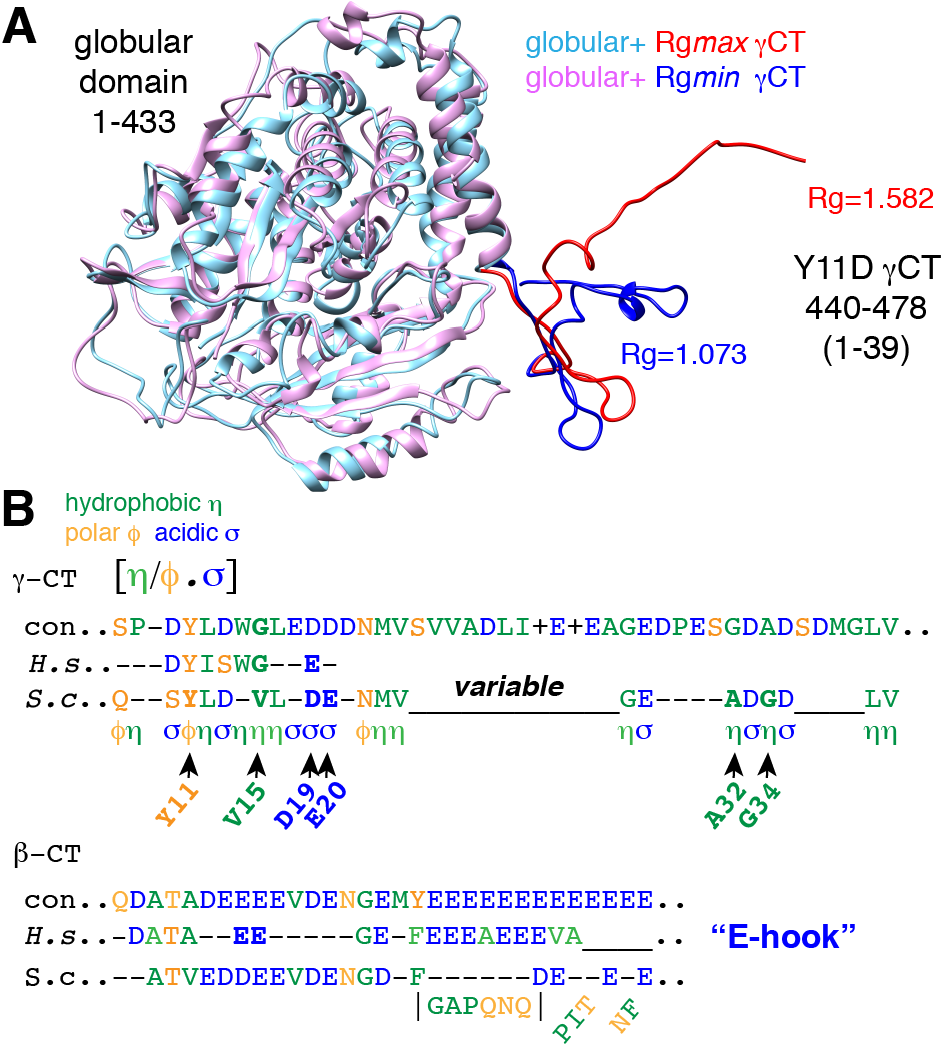
\includegraphics{figures/Figure_9.png}
\end{figure}

The CTs of $\alpha$- $\beta$- and $\gamma$-tubulins are enriched in acidic residues (Asp, Glu). \gct s across eukaryotes additionally contain clusters of hydrophobic or polar residues which are not found in $\alpha$- or $\beta$-CTs. Interestingly, the residues most broadened in Y11D NMR spectra, i.e. those most affected by the compact-to-extended transition (V15, D19, E20, A32, G34), are all found in positions conserved either on a sequence level or on a physical property level (polarity/charge) in a consensus \gct sequence(Fig. 9B). This suggests that clusters of hydrophobic residues, including those that contribute to transitions between compact and extended confor-mations in the S.c. D11 \gct, are a feature of an otherwise diverse set of \gct s across many eukaryotic organisms.  
